\documentclass{ieeeojies}
\usepackage{cite}
\usepackage{amsmath,amssymb,amsfonts}
\usepackage{algorithmic}
\usepackage{graphicx}
\usepackage{textcomp}
\usepackage{array}
\usepackage[table]{xcolor}
\usepackage{multirow}
\usepackage{multicol}
\usepackage{float}
% \usepackage{caption}
\usepackage[T1]{fontenc}
\def\BibTeX{{\rm B\kern-.05em{\sc i\kern-.025em b}\kern-.08em
    T\kern-.1667em\lower.7ex\hbox{E}\kern-.125emX}}

\begin{document}
\title{A Comparative Analysis of Machine Learning and Deep Learning Models for Real Estate Stock Market Forecasting}

\author{\uppercase{Phan Chi Cuong}\authorrefmark{1},
\uppercase{Nguyen Le Khang\authorrefmark{2}, and Le Pham Quoc Bao}\authorrefmark{3}}

\address[1]{Faculty of Information Systems, University of Information Technology, (e-mail: 21520673@gm.uit.edu.vn)}
\address[2]{Faculty of Information Systems, University of Information Technology, (e-mail: 21520960@gm.uit.edu.vn)}
\address[3]{Faculty of Information Systems, University of Information Technology, (e-mail: 21521849@gm.uit.edu.vn)}

\markboth
{Author \headeretal: Phan Chi Cuong, Nguyen Le Khang, Le Pham Quoc Bao}
{Author \headeretal: Phan Chi Cuong, Nguyen Le Khang, Le Pham Quoc Bao}

\begin{abstract}
  This study shows a detailed comparative analysis of statistical models, machine learning, and deep learning models for predicting real estate stock prices. We check the predictive capabilities of different models like the Autoregressive Integrated Moving Average with Exogenous variables (ARIMAX), Linear Regression, Long Short-Term Memory (LSTM) networks, Recurrent Neural Networks (RNN), Gated Recurrent Units (GRU), Random Forest (RF), Fast Fourier Transform (FFT), and TimesNet. Using a carefully prepared dataset of historical stock prices and technical indicators, we train and test these models with MAPE, RMSE and Mean Directional Accuracy (MDA). Our results show that deep learning models, like LSTM and GRU, perform better than traditional time series and machine learning models in catching the complex behaviors of real estate stock markets. Also, adding technical indicators as exogenous variables in ARIMAX, using frequency domain analysis with FFT, and applying Linear Regression all improve forecasting accuracy. This research gives useful insights for investors and financial analysts aiming to make informed decisions in the real estate stock market.
\end{abstract}

\begin{keywords}
  Placeholder
\end{keywords}

\titlepgskip=-15pt

\maketitle

\section{Introduction}
\label{sec:introduction}
Time-series forecasting is very important in decision-making across many fields. Its value comes from its ability to provide insights about future trends and patterns in time-dependent data. For example, accurate forecasting of stock prices, foreign exchange rates, and interest rates is crucial for making good financial investments. In healthcare, organizations depend on predictions of patient demand and resource use to optimize resources and improve patient care. Energy companies also use time-series forecasting to optimize energy production, distribution, and consumption. The accuracy and efficiency of time-series forecasting models greatly affect organizational performance and decision-making.

In this paper, we explore a new approach to make time-series forecasting better using the Fast Fourier Transform (FFT). The FFT algorithm extracts frequency-domain features from time-series data, offering a promising way to improve forecast accuracy and computational efficiency. Our investigation include a comparative analysis of models trained with FFT-based features against traditional time-domain features. We apply this method to predict stock prices of real estate companies, using not only FFT but also other techniques like TimesNet and Random Forest. Through our study, we highlight the interpretability of frequency-domain features and their relationship with underlying time-series patterns, emphasizing the potential of FFT-based feature engineering to improve forecasting models.

\section{Related Works}

In recent years, many stock prediction models have been researched and many articles have been published, such as: \\

Hind Daori, Alanoud Alanazi, Manar Alharthi, Ghaida Alzahrani (2022)\cite{b1} used Artificial Neural Network (ANN), Random Forest
Classifier, Logistic Regression,and then analyze and predict the
patterns of previous stock prices and the results showed that the models were efficient and produced better results.\\

Hugo Souto(2023) \cite{b2} has researched about TimesNet for Realized Volatility Prediction. Finally, they concluded that TimesNet stands out as a reliable and effective benchmark model for researching realized volatility. Although it may not always surpass NBEATSx and NHITS in every metric, its strong performance and consistency make it a valuable option, especially when compared to TFT. Overall, TimesNet presents a balanced and dependable choice that combines reliability with effectiveness, making it a suitable neural network model for researchers and practitioners in the field of realized volatility. \\

In another article by Bohumil Stádník, Jurgita Raudeliuniene, Vida Davidavičienė \cite{b3}, they pointed out that the Fourier analysis may not be advantageous for investors forecasting stock market prices as it fails to detect existing predominant cycles. An attempt to identify significant periods in the US stock market data using FFT, a method of Fourier analysis, proved to be unacceptable. Similar failures can be expected with other liquid investment instruments or financial data series. Despite this, Fourier analysis is still used for forecasting in finance and its benefits are a topic of discussion among financial market practitioners and academicians.


\section{Materials}
\subsection{Dataset}

The dataset comprises historical daily closing stock prices (in Vietnamese Dong - VND) for three prominent Vietnamese real estate companies:
 \\
  \indent\textbullet\ Quoc Cuong Gia Lai Joint Stock Company (QCG) \\
  \indent\textbullet\ Dat Xanh Group Joint Stock Company (DXG) \\
  \indent\textbullet\ Vinhomes Joint Stock Company (VHM) \\
  \\
The data spans a five-year period from March 1, 2019, to March 1, 2024.  While the raw data includes additional attributes such as opening price, high, low, volume, and change, this study focuses solely on the "Close" price to develop predictive models for future closing price movements.

\subsection{Descriptive Statistics}
\begin{table}[H]
  \centering
  \caption{QCG, VHM, DXG’s Descriptive Statistics}
\begin{tabular}{|>{\columncolor{blue!20}}c|c|c|c|}
    \hline
     \rowcolor{blue!20} & DXG & VHM & QCG \\ \hline
     Observations & 1252 & 1252 & 1252 \\ \hline
     Mean & 17676 & 17471.91 & 7586.17\\ \hline
     Median & 15348 & 15624 & 7105\\ \hline
     Std & 7862 & 7659 & 3102.55\\ \hline
     Min & 6739 & 6739 & 3320\\ \hline
     Max & 46750 & 46750 & 23200\\ \hline
     25\% & 12303 & 12260 & 4960\\ \hline
     50\% & 15348 & 15624 & 7105\\ \hline
     75\% & 20806 & 20262 & 9182.5\\ \hline
    Skewness & 1.41 & 1.49 & 1.13\\ \hline
    Kurtosis & 1.97 & 2.37 & 1.68\\ \hline

     
\end{tabular}
\end{table}
\begin{figure}[H]
  \centering
  \begin{minipage}{0.23\textwidth}
  \centering
  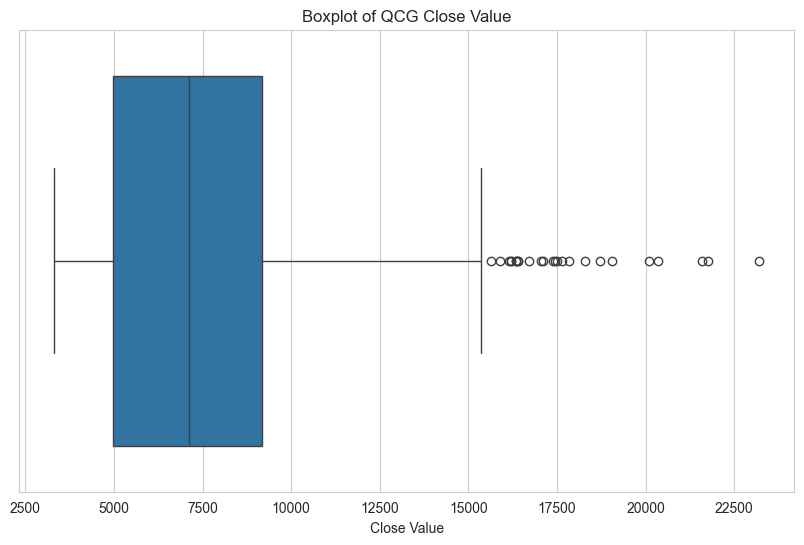
\includegraphics[width=1\textwidth]{bibliography/Figure/QCGboxplot.png}
  \caption{QCG stock price's boxplot}
  \label{fig:1}
  \end{minipage}
  \hfill
  \begin{minipage}{0.23\textwidth}
  \centering
  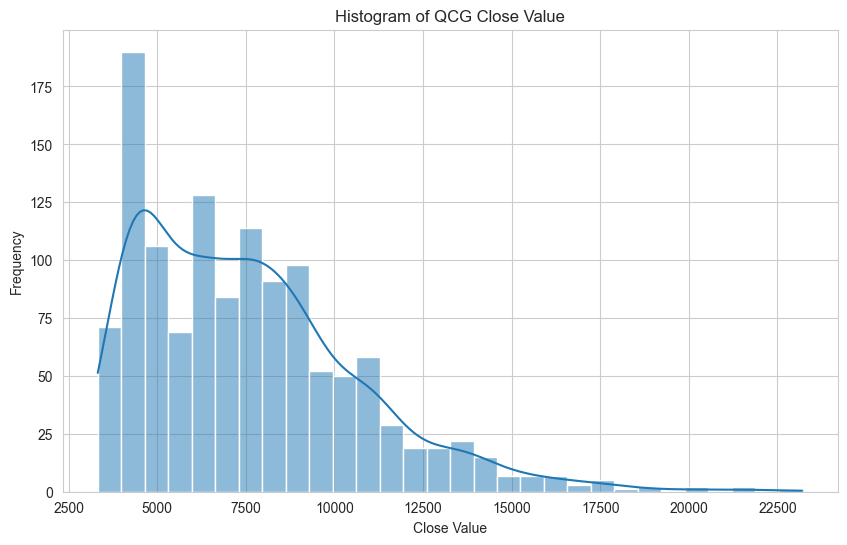
\includegraphics[width=1\textwidth]{bibliography/Figure/QCGhist.png}
  \caption{QCG stock price's histogram}
  \label{fig:2}
  \end{minipage}
\end{figure}
\begin{figure}[H]
  \centering
  \begin{minipage}{0.23\textwidth}
  \centering
  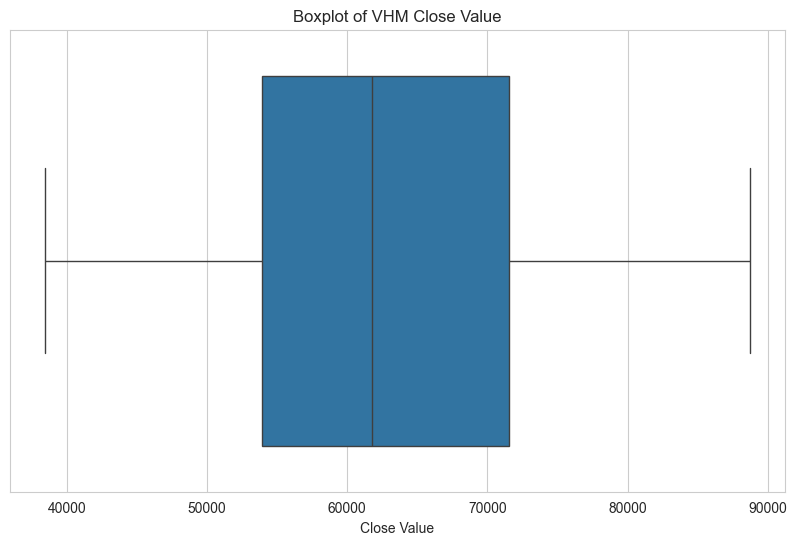
\includegraphics[width=1\textwidth]{bibliography/Figure/VHMBoxPlot.png}
  \caption{VHM stock price's boxplot}
  \label{fig:1}
  \end{minipage}
  \hfill
  \begin{minipage}{0.23\textwidth}
  \centering
  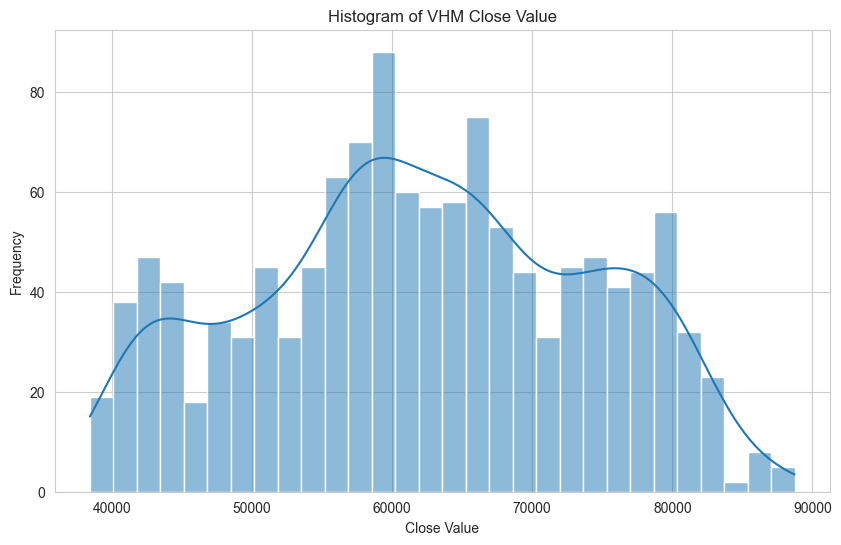
\includegraphics[width=1\textwidth]{bibliography/Figure/VHMhist.png}
  \caption{VHM stock price's histogram}
  \label{fig:2}
  \end{minipage}
\end{figure}

\begin{figure}[H]
  \centering
  \begin{minipage}{0.23\textwidth}
  \centering
  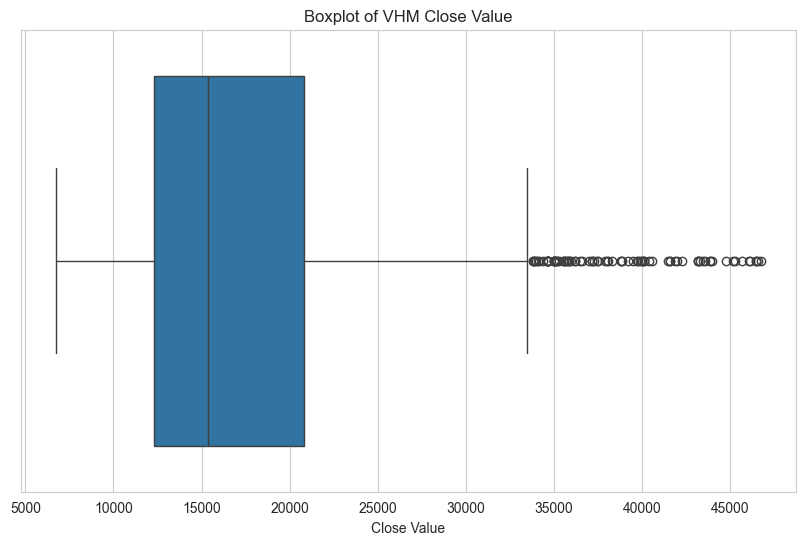
\includegraphics[width=1\textwidth]{bibliography/Figure/DXGBoxPlot.png}
  \caption{DXG stock price's boxplot}
  \label{fig:1}
  \end{minipage}
  \hfill
  \begin{minipage}{0.23\textwidth}
  \centering
  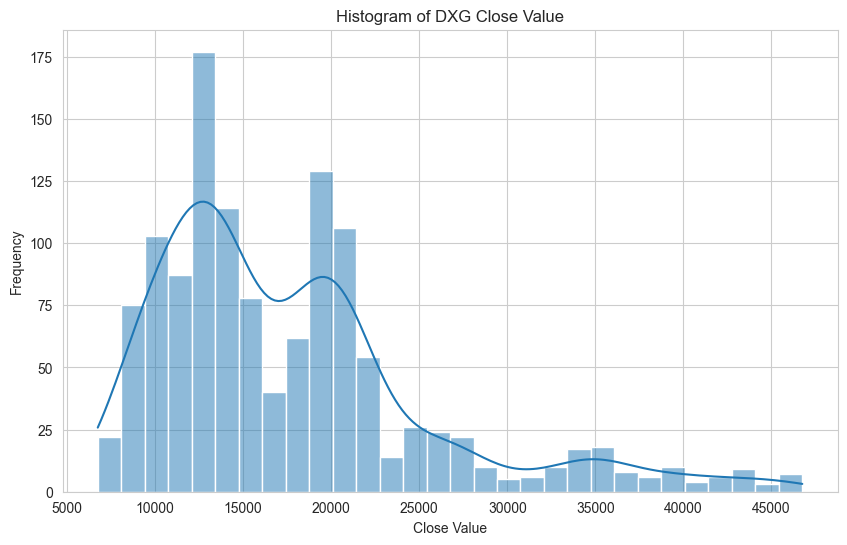
\includegraphics[width=1\textwidth]{bibliography/Figure/DXGHistogram.png}
  \caption{DXG stock price's histogram}
  \label{fig:2}
  \end{minipage}
\end{figure}


\section{Methodology}
\subsection{Data Preprocessing}
The initial dataset of daily closing stock prices was incomplete, lacking data for weekends and potentially other non-trading days, resulting in a non-consecutive time series. Recognizing the importance of a continuous time series for accurate analysis, we took steps to fill these gaps. We assumed that the market doesn't experience significant changes over non-trading days and used the closing price of the preceding Friday to fill the missing values for weekends and holidays.

Furthermore, to enhance the predictive power of our models, we calculated several technical indicators from the closing prices. These indicators included Simple Moving Average (SMA), Exponential Moving Average (EMA), Relative Strength Index (RSI), Moving Average Convergence Divergence (MACD), Bollinger Bands (BB), Average True Range (ATR), and On-Balance Volume (OBV). These widely-used indicators provide valuable information about market trends, momentum, and volatility, serving as potential predictors in our linear regression model.

By addressing the missing data and incorporating technical indicators, we created a more comprehensive and informative dataset for our subsequent analysis. This enhanced dataset enabled us to explore the relationships between stock prices and various market factors, ultimately contributing to the development of more accurate predictive models.
\subsection{Linear Regression}
A linear regression model was employed to analyze the relationship between the closing price of real estate company stocks and various technical indicators. Linear regression is a statistical method that models the linear relationship between a dependent variable and one or more independent variables. In this context, the closing price of real estate stocks was chosen as the dependent variable, while several technical indicators derived from the stock's price and volume data were considered as potential independent variables.

The mathematical representation of a multiple linear regression model is as follows:
\[Y=\beta_0+\beta_1X_1+\beta_2X_2+\cdots+\beta_kX_k+\varepsilon\]
Where:\\
	\indent\textbullet\ Y is the predicted closing price of the real estate stock. \\
	\indent\textbullet\ \(X_1, X_2, \ldots, X_k\) are the independent (explanatory) variables.\\
	\indent\textbullet\ \(\beta_0\) is the intercept term.\\
	\indent\textbullet\ \(\beta_1,..., \beta_k\) are the regression coefficients for the independent variables.\\
	\indent\textbullet\ \(\varepsilon\) is the error term.
  
  The dataset used for this analysis included stock price data for various real estate companies, spanning a specific time period. The dataset included various technical indicators such as Simple Moving Average (SMA), Exponential Moving Average (EMA), Relative Strength Index (RSI), Moving Average Convergence Divergence (MACD), Bollinger Bands (BB\_High, BB\_Middle, BB\_Low), Average True Range (ATR), and On-Balance Volume (OBV). These indicators were selected as potential independent variables due to their established relevance in technical stock analysis.
\subsection{Random Forest}
Random forest is a supervised learning algorithm. The “forest” it builds is an ensemble of decision trees, usually trained with the bagging method. The general idea of the bagging method is that a combination of learning models increases the overall result.
\begin{figure}[H]
  \centering
  \begin{minipage}{0.8\linewidth}
  \centering

  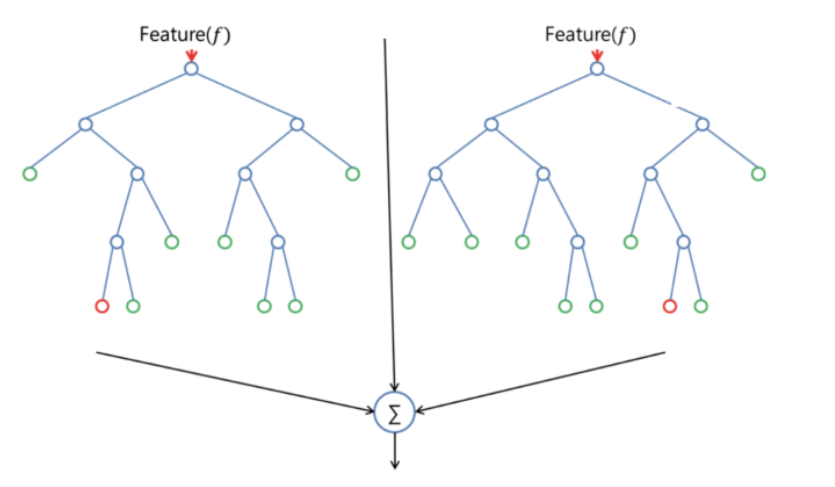
\includegraphics[width=1\textwidth]{bibliography/Figure/RF_work.png}
  \caption{Random forest models}
  \label{fig:1}
  \end{minipage}
\end{figure}
Despite its complexity and computational intensity, Random Forest effectively reduces overfitting and enhances prediction performance, making it a powerful and versatile machine learning algorithm.
\subsection{GRU}
GRU is a simplified version of LSTM (Long Short-Term Memory) and has fewer parameters, which helps reduce the time and computational resources required during model training.
The structure of GRU consists of two main gates:
\\
\indent\textbullet\ Update Gate: Controls the amount of information from the previous hidden state that needs to be carried over to the current state.
\[
z_t = \sigma(W_z \cdot [h_{t-1}, x_t] + b_z)
\]
\indent\textbullet\  Reset Gate: Decides how much of the past information to forget. \\
\[
r_t = \sigma(W_r \cdot [h_{t-1}, x_t] + b_r)
\]
\indent\textbullet\ Current memory content : determines the potential contribution to the updated hidden state.\\
\[
\tilde{h}_t = \tanh(W_h \cdot [r_t \odot h_{t-1}, x_t] + b_h)
\]
\indent\textbullet\ Final memory at current time step : is the updated hidden state that combines the previous hidden state and the new candidate hidden state based on the update gate's decision. This updated hidden state effectively balances retaining information from the past and incorporating new information from the current time step.\\
\[
h_t = (1 - z_t) \odot h_{t-1} + z_t \odot \tilde{h}_t
\]
Where:
\begin{itemize}
  \item \( h_t \) is the final hidden state at time step \( t \).
  \item \( z_t \) is the update gate vector at time step \( t \).
  \item \( h_{t-1} \) is the hidden state from the previous time step \( t-1 \).
  \item \( \tilde{h}_t \) is the candidate hidden state at time step \( t \).
  \item \( \odot \) represents element-wise multiplication. This operation is applied element-wise to vectors or matrices.
  \item \( 1 - z_t \) is the complement of the update gate vector.
\end{itemize}


\begin{figure}[ht]
\centering
  \begin{minipage}{0.5\textwidth}
    \centering
    % \includegraphics[width=\textwidth]{bibliography/Figure/correlation_arimax.png}
    \caption{Correlation Matrix of Filtered Data}
    \label{tab:correlation_matrix}
  \end{minipage}
\end{figure}


The model was then trained using the preprocessed dataset, and its performance was evaluated using appropriate metrics such as Mean Squared Error (MSE), R-squared, and adjusted R-squared.

The choice of independent variables for the final model was guided by the correlation matrix (Figure~\ref{tab:correlation_matrix}), which revealed the strength and direction of linear relationships between the closing price and each indicator. Variables exhibiting higher correlation with the closing price were considered more influential and were prioritized for inclusion in the model.

By analyzing the estimated coefficients (\( \beta_1, \beta_2, ..., \beta_n \)) of the linear regression model, we can quantify the impact of each technical indicator on the predicted closing price of real estate stocks. This analysis provides valuable insights into the factors that drive the stock's price movements and can inform investment decisions.
  \subsection{ARIMAX}
  Stock prices, much like weather patterns, exhibit both inherent trends and reactions to external forces. To capture this duality, we employed an Autoregressive Integrated Moving Average with Exogenous variables (ARIMAX) model. Building upon the established ARIMA framework, ARIMAX allows us to weave external factors, or "exogenous variables," into our forecasting tapestry.
  Mathematically, the ARIMAX model is expressed as:
  
  \[y(t) = \alpha + \sum_{i=1}^{p} \beta_i y(t-i) + \sum_{j=1}^{q} \phi_j \varepsilon(t-j) + \sum_{k=1}^{r} \gamma_k x_k(t) + \varepsilon(t)\]
In our context, $y(t)$ represents the real estate stock price at time (t). The terms  $(\sum_{i=1}^{p} \beta_i y(t-i))$ and $(\sum_{j=1}^{q} \phi_j \varepsilon(t-j))$ capture the autoregressive (AR) and moving average (MA) components, respectively, similar to ARIMA. The added dimension lies in $(\sum_{k=1}^{r} \gamma_k x_k(t))$, where $x_k(t)$ are our carefully curated exogenous variables, namely the technical indicators derived from our preprocessed dataset.

The selection of the ARIMAX model's parameters – the number of AR and MA terms, the order of differencing, and the specific exogenous variables – was a meticulous process. It involved scrutinizing autocorrelation and partial autocorrelation plots, along with consulting information criteria like AIC and BIC.

With the model's architecture finalized, we trained it on our refined dataset, where the closing prices served as the main melody, and the technical indicators provided the counterpoint. We assessed the model's performance using various metrics, including Mean Absolute Error (MAE), Mean Squared Error (MSE), Root Mean Squared Error (RMSE), and Mean Absolute Percentage Error (MAPE), seeking to minimize these measures of forecasting error.

This ARIMAX model, enriched by the inclusion of exogenous variables, allowed us to not only decipher the inherent rhythm of real estate stock prices but also to anticipate their movements based on the external influences captured by the technical indicators. It represents a step towards a more holistic understanding of the stock market's complex dance.


  \subsection{RNN}
  Recurrent Neural Networks (RNNs) are a class of artificial neural networks designed to recognize patterns in sequences of data, such as text, time series data, and speech. Unlike traditional feedforward neural networks, RNNs have connections that form directed cycles, allowing information to persist. This characteristic enables RNNs to exhibit temporal dynamic behavior, making them suitable for tasks where context and sequential data play a critical role.
  \\ The core concept behind Recurrent Neural Networks (RNNs) is the introduction of a hidden state that captures information about previous inputs. This hidden state is updated at each time step as new inputs are processed. Mathematically, this process can be represented as follows:
  \[
  h_t = \sigma(W_h \cdot h_{t-1} + W_x \cdot x_t + b)
  \]
  where:
  \begin{itemize}
      \item $h_t$ is the hidden state at time $t$.
      \item $W_h$ and $W_x$ are weight matrices.
      \item $x_t$ is the input at time $t$.
      \item $b$ is the bias term.
      \item $\sigma$ is a non-linear activation function (e.g., $\tanh$ or $\text{ReLU}$).
  \end{itemize}  
  % LSTM Introduction
  \subsection{Long Short Term Memory (LSTM)}

   Long Short Term Memory networks (LSTM), often known as LSTMs, are a special type of recurrent neural network (RNN) with the ability to learn and remember long-term dependencies. LSTMs were introduced by Hochreiter and Schmidhuber in 1997, and have since been refined and developed further by many researchers and experts in the field. Thanks to their exceptional performance on various tasks, LSTMs have become increasingly popular.

  LSTMs are designed to address the problem of long-term dependencies. Retaining information over extended periods is an inherent characteristic of LSTMs, requiring no special training to achieve this capability. In other words, the ability to remember long-term information is built into LSTMs.

  Unlike traditional RNNs, which have a simple structure with a single tanh activation layer, LSTMs have a more complex chain-like structure, with modules that contain up to four layers interacting in a special way.

  \noindent 
  \textbf{In the \(t\)-th state of the LSTM model:}

\textbf{Output}: \(c_t\), \(h_t\), where \(c\) is the cell state, and \(h\) is the hidden state.

\textbf{Input}: \(c_{t-1}\), \(h_{t-1}\), \(x_t\), where \(x_t\) is the input at state \(t\) of the model, and \(c_{t-1}\) and \(h_{t-1}\) are the outputs from the previous layer. The hidden state \(h\) is similar to \(s\) in RNN, while \(c\) is the unique aspect of LSTM.

\textbf{Reading the diagram}: The symbols \(\sigma\) and tanh indicate that the step uses the sigmoid and tanh activation functions, respectively. The multiplication is element-wise, and the addition is matrix addition.

\textbf{Gates}: \(f_t\), \(i_t\), \(o_t\) correspond to the forget gate, input gate, and output gate, respectively.

\begin{figure}[H]
  \centering
  \begin{minipage}{0.5\textwidth}
    \centering
    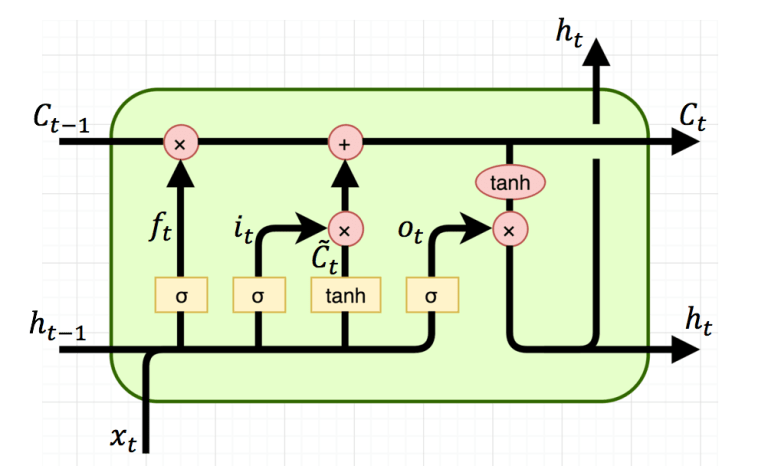
\includegraphics[width=\textwidth]{bibliography/Figure/LSTM Model.png}
    \caption{LSTM Model}
    \label{fig:1}
  \end{minipage}
\end{figure}



\noindent \textbullet \textbf{ Forget gate}:
\[
f_t = \sigma(U_f \cdot x_t + W_f \cdot h_{t-1} + b_f)
\]

\noindent \textbullet \textbf{ Input gate}:
\[
i_t = \sigma(U_i \cdot x_t + W_i \cdot h_{t-1} + b_i)
\]

\noindent \textbullet \textbf{ Output gate}:
\[
o_t = \sigma(U_o \cdot x_t + W_o \cdot h_{t-1} + b_o)
\]

Thus, the expressions for each gate of the LSTM illustrate how each gate manages the information flowing in and out of the model's states.


  % TimesNet Introduction
  \subsection{TimesNet}
  TimesNet is a recent advancement in machine learning designed specifically for time series analysis tasks. Developed by researchers at Shanghai Jiao Tong University, it tackles the core challenge of capturing temporal variations within data.

  \textbf{Core Idea: Transforming 1D Time Series to 2D Space}

  \noindent
  Traditional time series models handle data as a single-dimensional sequence. TimesNet breaks this mold by introducing a transformation step. It converts the 1D data into a 2D tensor. This allows the model to capture complex relationships between data points, including both cyclical and inter-cyclical variations.
  
  \textbf{The Building Block: TimesBlock}

  \noindent
  The core building block of TimesNet is the TimesBlock. It is a module that performs the following:

  \textbf{Inception Block}: This block, inspired by the Inception architecture used in image recognition, efficiently extracts features from the transformed 2D tensor. It uses multiple filter sizes within a single layer, allowing it to capture patterns at different scales within the data.

  \indent
  \textbf{Adaptive Multi-Periodicity Discovery}: TimesNet does not require pre-defining the cyclical patterns in the data. The TimesBlock can automatically discover these periodicities within the 2D representation. This makes TimesNet adaptable to various time series data with different inherent periodicities.
  \subsection{Fast Fourier Transform Forecasting Model (FFT)}
  The fast Fourier transform (FFT) is a computational tool that transforms time-domain data into the frequency domain by deconstructing the signal into its individual parts: sine and cosine waves. This computation allows engineers to observe the signal’s frequency components rather than the sum of those components.
  \\ 
  The FFT forecasting model leverages the fact that any periodic time series can be represented as a sum of sinusoidal functions (sines and cosines) of different frequencies. By transforming the time series data into the frequency domain, we can isolate significant frequencies that capture the underlying periodic patterns.
 \\
 Given a time series \( x(t) \), the Fast Fourier Transform (FFT) converts it into the frequency domain \( X(f) \):

\[
X(f) = \sum_{t=0}^{N-1} x(t) e^{-i 2\pi ft / N}
\]

where:
\begin{itemize}
    \item \( N \) is the number of data points.
    \item \( f \) represents different frequency components.
\end{itemize}
To reconstruct the time series from significant frequencies:

\[
x(t) = \sum_{f \in F} X(f) e^{i 2\pi ft / N}
\]

where \( F \) is the set of significant frequencies.
\\\\
The Fast Fourier Transform Forecasting Model is a powerful tool for analyzing and forecasting time series data with periodic components. By transforming data into the frequency domain, it enables the identification of significant patterns and trends, offering an efficient and effective approach to time series forecasting.
\section{Result}
Placeholder line
\subsection{Evaluation Methods}
\textbf{Mean Percentage Absolute Error} (MAPE): is the average percentage error in a set of predicted values.\\
\[MAPE=\frac{100\%}{n}  \sum_{i=1}^{n} |y_i-\hat{y_i} |  = 1 \]\\
\textbf{Root Mean Squared Error} (RMSE): is the square root of average value of squared error in a set of predicted values.\\
\[RMSE=\sqrt{\sum_{i=1}^{n} \frac{(\hat{y_i}-y_i )^2}{n} }\]\\
\textbf{Mean Absolute Error} (MAE):is the relative difference between the log-transformed actual and predicted values.\\
\[
MAE = \frac{1}{n} \sum_{i=1}^{n} \left| \hat{y}_i - y_i \right|
\]

where:
\begin{itemize}
    \item \(n\) is the number of observations.
    \item \(\hat{y}_i\) represents the predicted values.
    \item \(y_i\) represents the actual values.
\end{itemize}
\subsection{DXG Dataset} 
\begin{table}[H]
  \centering
  \begin{tabular}{|c|c|c|c|c|}
         \hline
         \multicolumn{5}{|c|}{\textbf{DXG Dataset's Evaluation}}\\
         \hline
         \centering Model & Training:Testing & RMSE & MAPE (\%) & MAE\\
         \hline
         \multirow{2}{*}{LR} & 7:3 & 1023.75 & 5.06 & 748.41 \\ & 8:2 & 950.44 & 4.06 & 707.96 \\ & \textbf{9:1} & \textbf{843.98} & \textbf{3.25} & \textbf{579.74}\\
         \hline
         \multirow{2}{*}{ARIMA} & 7:3&11864.3&7.52&0.021\\ & 8:2&8521.33&5.01&0.009 \\ & \textbf{9:1} & \textbf{7006.54} & \textbf{3.73} & \textbf{0.006}\\
         \hline
         \multirow{2}{*}{GRU} & \textbf{7:3}& \textbf{715.7} & \textbf{1.015} & \textbf{513.7} \\ & 8:2 & 759.27 & 1.013 & 534.78  \\ & 9:1 & 743.16	&0.969&507.51\\
         \hline
         \multirow{2}{*}{RNN} & 7: &  719.14 &  0.99 &  500.41 \\ & 8:2 &  1159.64 & 1.765 &  932.25 \\ & \textbf{9:1} & \textbf{663.95} & \textbf{0.886} & \textbf{464.22} \\
         \hline
         \multirow{2}{*}{RF} & \textbf{7:3}	& \textbf{743} & \textbf{1.06} &  \textbf{537.83} \\ & 8:2 & 823.04 & 1.164 & 612.98 \\ & 9:1 & 794 & 1.071 & 562.85\\
         \hline
         \multirow{2}{*}{LSTM} & 7:3 & 289.96 & 2.81 & 215.99 \\ & \textbf{8:2} & \textbf{330.30} & \textbf{3.15} & \textbf{244.18} \\ & 9:1 & 317.71	&3.08&239.83\\
         \hline
         \multirow{2}{*}{TimesNet} & \textbf{7:3} & \textbf{4344.14} & \textbf{25.61} & \textbf{3567.59} \\ & 8:2 & 3370.33 & 18.06 & 2613.58 \\ & 9:1 & 1668.46	& 6.20 &1231.19\\
         \hline
         \multirow{2}{*}{FFT} & 7:3 & 941.7588 &  1.7384 &  0.0005 \\ & 8:2 & 939.7588 &  1.6546 &  0.0005 \\ & \textbf{9:1} & \textbf{936.8374} & \textbf{1.6273} & \textbf{0.0005}\\
         \hline
    \end{tabular}
    \caption{DXG Dataset's Evaluation}

    \label{vcbresult}
\end{table}
\begin{figure}[H]
  \centering
  \begin{minipage}{0.23\textwidth}
  \centering
  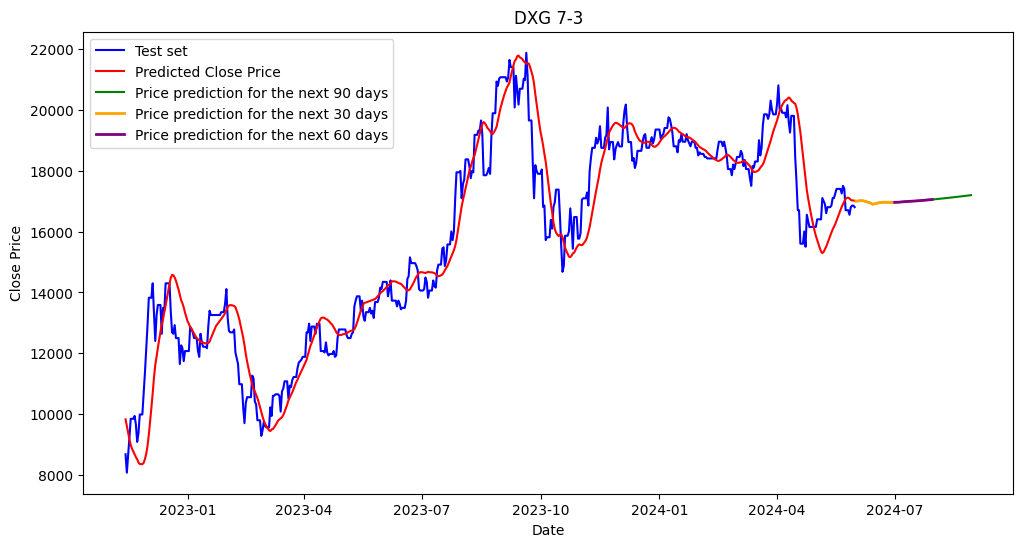
\includegraphics[width=1\textwidth]{bibliography/Figure/LR_DXG(7-3).png}
  \caption{LR  model's result with 7:3 splitting proportion}
  \label{fig:1}
  \end{minipage}
  \hfill
  \begin{minipage}{0.23\textwidth}
  \centering
  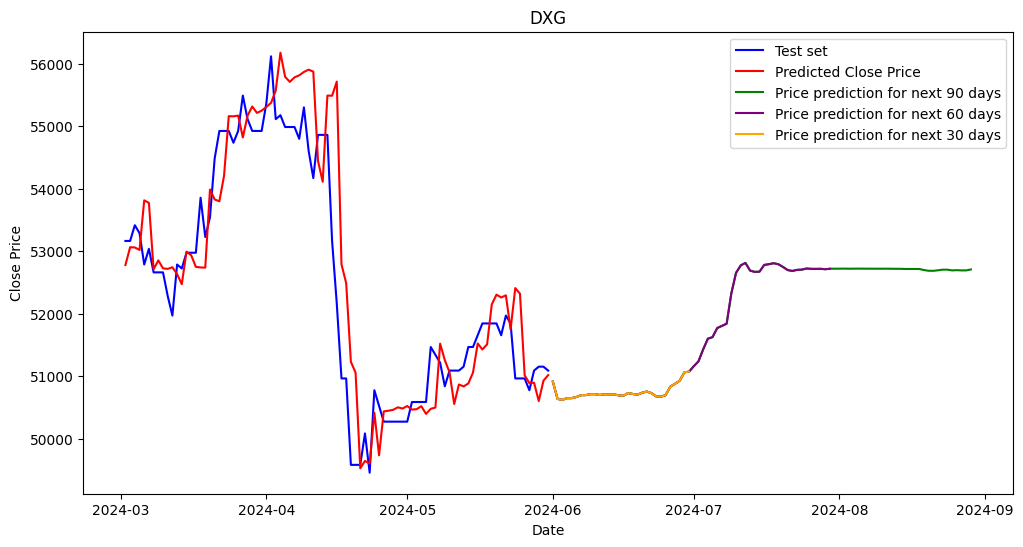
\includegraphics[width=1\textwidth]{bibliography/Figure/RNN_9-1.png}
  \caption{RNN model's result with 9:1 splitting proportion}
  \label{fig:2}
  \end{minipage}
\end{figure}
\begin{figure}[H]
  \centering
  \begin{minipage}{0.23\textwidth}
  \centering
  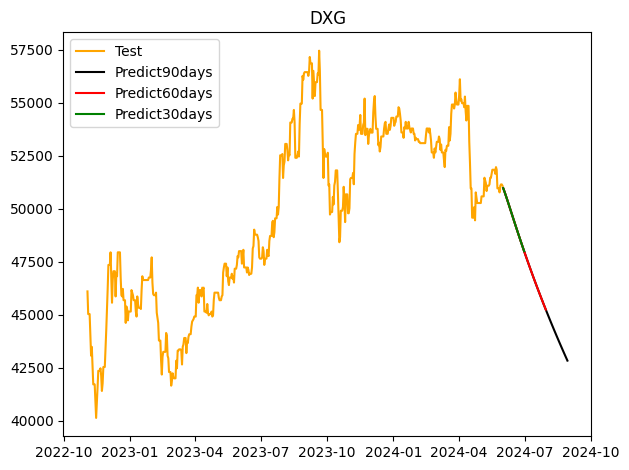
\includegraphics[width=1\textwidth]{bibliography/Figure/GRU_7-3.png}
  \caption{GRU model's result with 7:3 splitting proportion}
  \label{fig:1}
  \end{minipage}
  \hfill
  \begin{minipage}{0.23\textwidth}
  \centering
  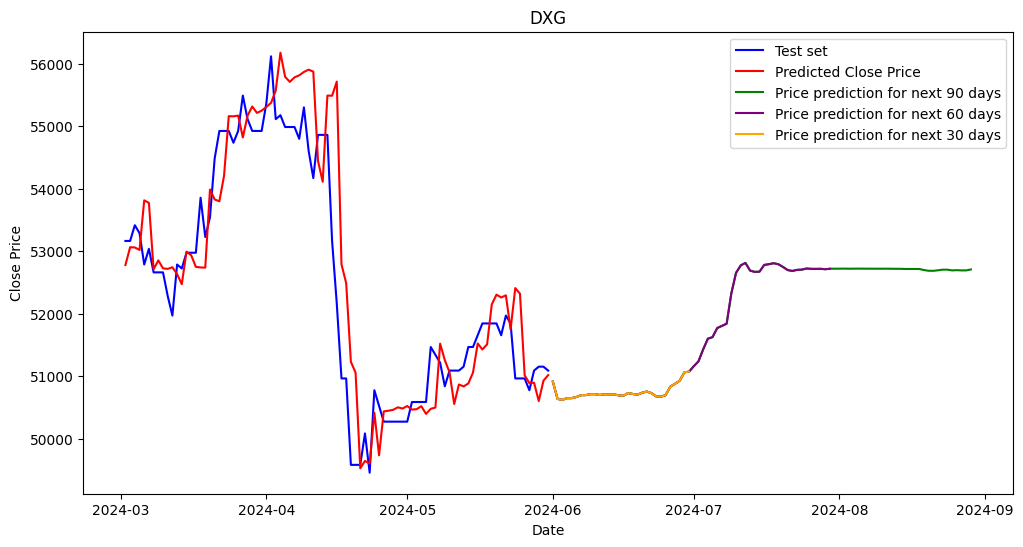
\includegraphics[width=1\textwidth]{bibliography/Figure/RNN_9-1.png}
  \caption{RNN model's result with 9:1 splitting proportion}
  \label{fig:2}
  \end{minipage}
\end{figure}
\begin{figure}[H]
  \centering
  \begin{minipage}{0.23\textwidth}
  \centering
  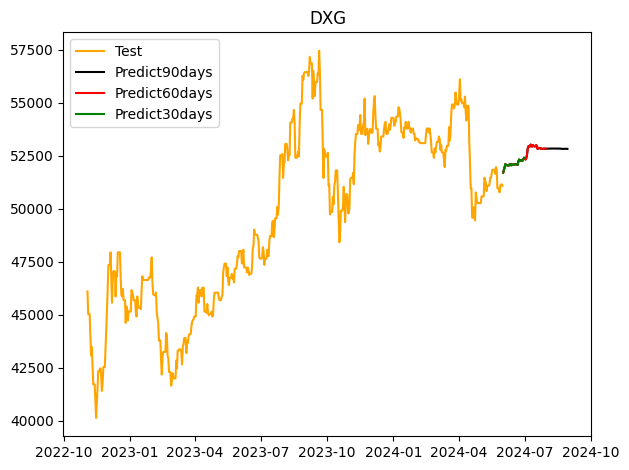
\includegraphics[width=1\textwidth]{bibliography/Figure/RF_7-3.png}
  \caption{RF model's result with 7:3 splitting proportion}
  \label{fig:1}
  \end{minipage}
  \hfill
  \begin{minipage}{0.23\textwidth}
  \centering
  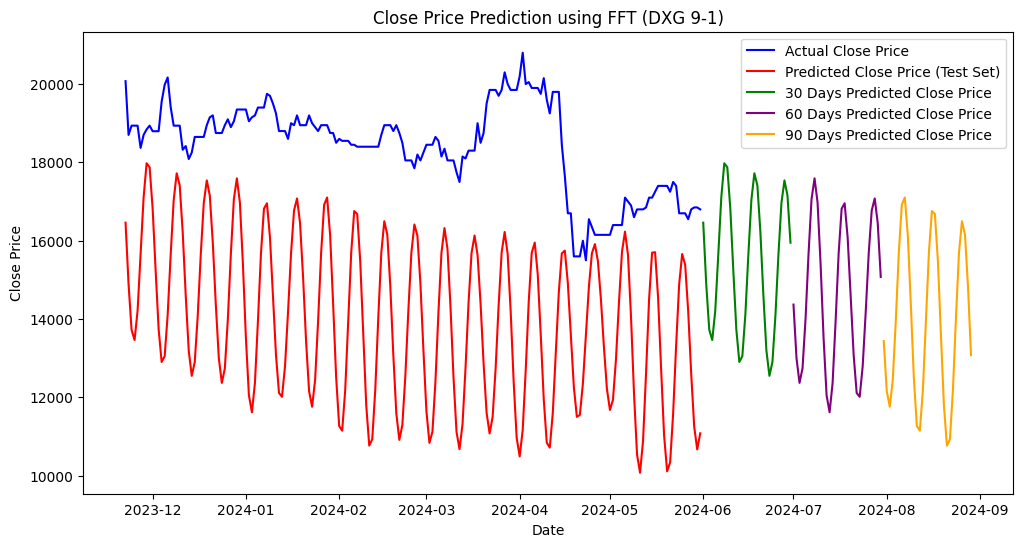
\includegraphics[width=1\textwidth]{bibliography/Figure/FFT_DXG(9-1).png}
  \caption{FFT model's result with 9:1 splitting proportion}
  \label{fig:2}
  \end{minipage}
\end{figure}


\subsection{VHM dataset} 

  \begin{table}[H]
    \centering
    \begin{tabular}{|c|c|c|c|c|}
           \hline
           \multicolumn{5}{|c|}{\textbf{VHM Dataset's Evaluation}}\\
           \hline
           \centering Model & Training:Testing & RMSE & MAPE (\%) & MAE\\
           \hline
           \multirow{2}{*}{LR} & 7:3 & 2291.01 & 3.71 & 1763.66 \\ & 8:2 & 1815.25 & 3.04 & 1414.67 \\ & \textbf{9:1} & \textbf{1220.21} & \textbf{2.36} & \textbf{988.38}\\
           \hline
           \multirow{2}{*}{ARIMA} & 7:3&11864.3&7.52&0.021\\ & 8:2&8521.33&5.01&0.009 \\ & \textbf{9:1} & \textbf{7006.54} & \textbf{3.73} & \textbf{0.006}\\
           \hline
           \multirow{2}{*}{GRU} & \textbf{7:3} & \textbf{1199.35} & \textbf{1.726} & \textbf{816.59} \\ & 8:2 &  1383.71 & 1.59 &678.3 \\ & 9:1 & 1412.4	&1.54&437.64\\
           \hline
           \multirow{2}{*}{RNN} & 7:3 &  1433.18 &  2.451 & 1123.99 \\ & 8:2 &  1027.73 & 1.638 &  712.2\\ & \textbf{9:1} & \textbf{538.78} & \textbf{0.868} & \textbf{362.53} \\
           \hline
           \multirow{2}{*}{RF} & 7:3	& 1751.89 & 5.53 &  416.56 \\ & 8:2 & 1460.66 & 2.67 & 1128.53 \\ & \textbf{9:1} & \textbf{879.48} & \textbf{1.82} & \textbf{759.41}\\
           \hline
           \multirow{2}{*}{LSTM} & 7:3 & 669.02 & 9.18 & 517.60 \\ & \textbf{8:2} & \textbf{703.27} & \textbf{10.10} & \textbf{558.62} \\ & 9:1 & 619.56	&7.93&480.60\\
           \hline
           \multirow{2}{*}{TimesNet} & \textbf{7:3} & \textbf{8752.95} & \textbf{13.01} & \textbf{6901.65} \\ & 8:2 & 8731.15 & 12.68 & 6713.77 \\ & 9:1 & 4092.95	& 6.36 &2913.35\\
           \hline
           \multirow{2}{*}{FFT} & 7:3 & 941.7588 &  1.7384 &  0.0005 \\ & 8:2 & 939.7588 &  1.6546 &  0.0005 \\ & \textbf{9:1} & \textbf{936.8374} & \textbf{1.6273} & \textbf{0.0005}\\
           \hline
      \end{tabular}
      \caption{VHM Dataset's Evaluation}
      \label{vcbresult}
  \end{table}

  \begin{figure}[H]
    \centering
    \begin{minipage}{0.23\textwidth}
    \centering
    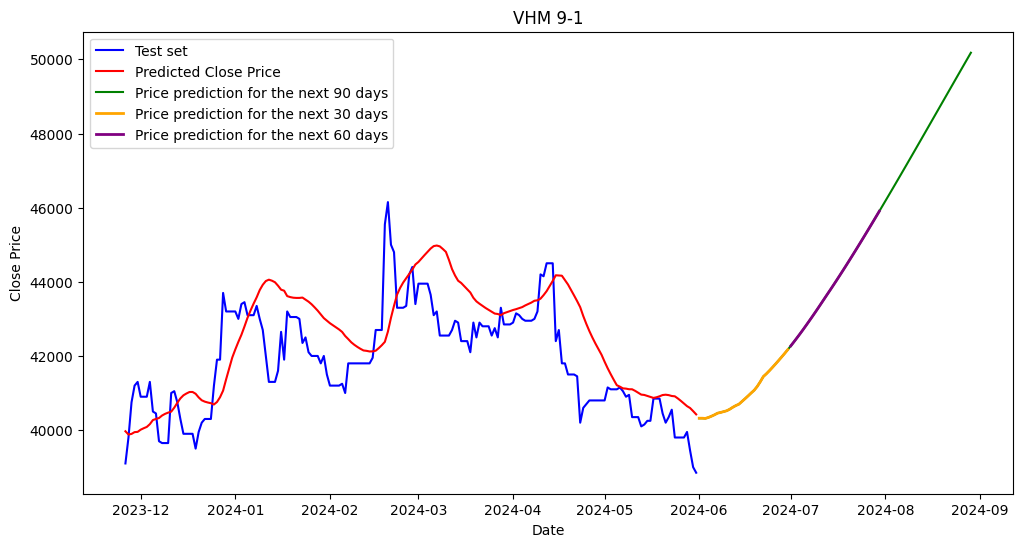
\includegraphics[width=1\textwidth]{bibliography/Figure/LR_VHM(9-1).png}
    \caption{LR model's result with 9:1 splitting proportion}
    \label{fig:1}
    \end{minipage}
    \hfill
    \begin{minipage}{0.23\textwidth}
    \centering
    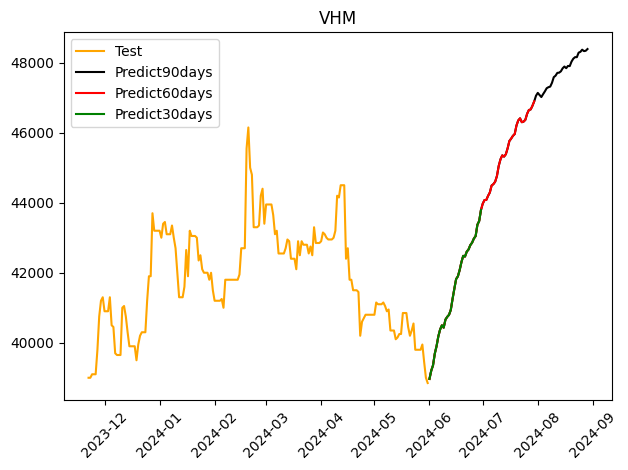
\includegraphics[width=1\textwidth]{bibliography/Figure/VHMRNN_9-1.png}
    \caption{RNN model's result with 9:1 splitting proportion}
    \label{fig:2}
    \end{minipage}
  \end{figure}
  \begin{figure}[H]
    \centering
    \begin{minipage}{0.23\textwidth}
    \centering
    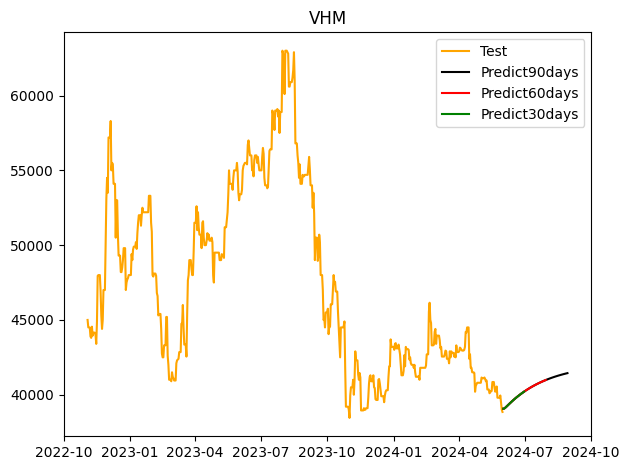
\includegraphics[width=1\textwidth]{bibliography/Figure/VHMGRU_7-3.png}
    \caption{GRU model's result with 7:3 splitting proportion}
    \label{fig:1}
    \end{minipage}
    \hfill
    \begin{minipage}{0.23\textwidth}
    \centering
    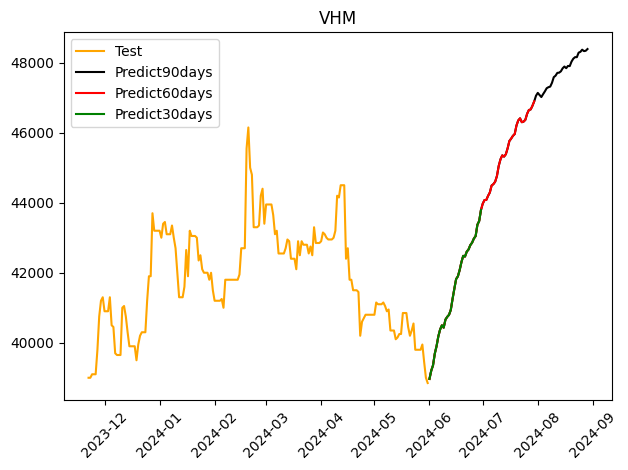
\includegraphics[width=1\textwidth]{bibliography/Figure/VHMRNN_9-1.png}
    \caption{RNN model's result with 9:1 splitting proportion}
    \label{fig:2}
    \end{minipage}
  \end{figure}

  \begin{figure}[H]
    \centering
    \begin{minipage}{0.23\textwidth}
    \centering
    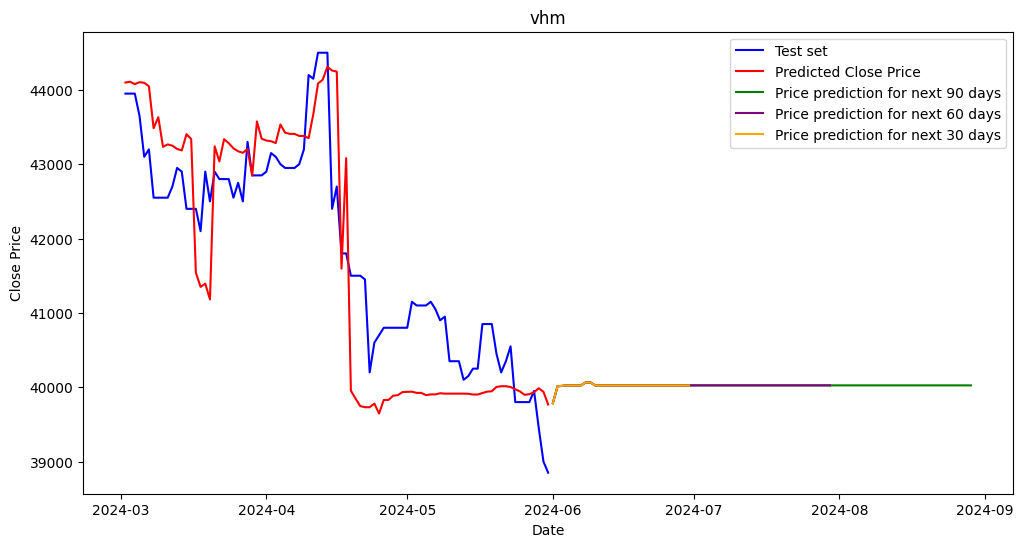
\includegraphics[width=1\textwidth]{bibliography/Figure/VHMRF_9-1.png}
    \caption{RF model's result with 9:1 splitting proportion}
    \label{fig:1}
    \end{minipage}
    \hfill
    \begin{minipage}{0.23\textwidth}
    \centering
    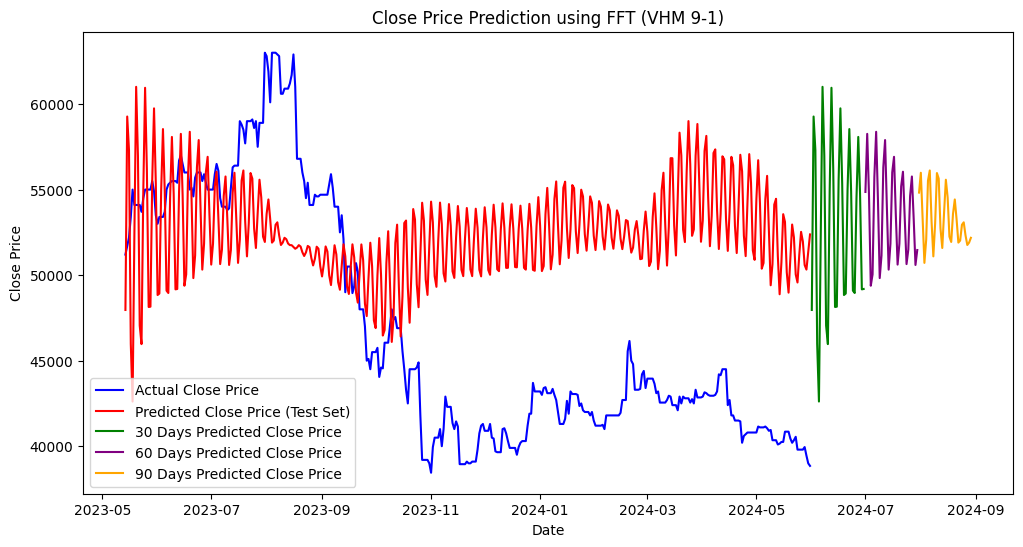
\includegraphics[width=1\textwidth]{bibliography/Figure/FFT_VHM(9-1).png}
    \caption{FFT model's result with 9:1 splitting proportion}
    \label{fig:2}
    \end{minipage}
  \end{figure}
  
\subsection{QCG dataset} 
\begin{table}[H]
  \centering
  \begin{tabular}{|c|c|c|c|c|}
         \hline
         \multicolumn{5}{|c|}{\textbf{QCG Dataset's Evaluation}}\\
         \hline
         \centering Model & Training:Testing & RMSE & MAPE (\%) & MAE\\
         \hline
         \multirow{2}{*}{LR} & 7:3 & 1023.74 & 5.05 & 748.41 \\ & 8:2 & 1036.14 & 7.10 & 781.55 \\ & \textbf{9:1} & \textbf{794.24} & \textbf{4.27} & \textbf{536.38}\\
         \hline
         \multirow{2}{*}{ARIMA} & 7:3&11864.3&7.52&0.021\\ & 8:2&8521.33&5.01&0.009 \\ & \textbf{9:1} & \textbf{7006.54} & \textbf{3.73} & \textbf{0.006}\\
         \hline
         \multirow{2}{*}{GRU} & 7:3 & 708.29 & 0.974 & 492.8\\ & 8:2 & 786.29 & 1.023 & 539.05  \\ & \textbf{9:1} & \textbf{665}	& \textbf{0.835} &  \textbf{437.64} \\
         \hline
         \multirow{2}{*}{RNN} & 7:3 &  777.04 &  1.113 & 561.96 \\ & 8:2 &  757.27 & 0.998 &  527.08\\ & \textbf{9:1} & 698.83 & 10043 & 527.0\\
         \hline
         \multirow{2}{*}{RF} & \textbf{7:3}	& \textbf{461.24} & \textbf{1.698} & \textbf{983.65} \\ & 8:2 & 1479.93 & 1.709 & 1046.63 \\ & 9:1 & 2378.81 &  2.51 & 1686.66\\
         \hline
         \multirow{2}{*}{LSTM} & \textbf{7:3} & \textbf{379.56} & \textbf{3.95} & \textbf{298.40} \\ & 8:2 & 314.71 & 2.84 & 216.48 \\ & 9:1 & 315.31	&2.41&200.57\\
         \hline
         \multirow{2}{*}{TimesNet} & \textbf{7:3} & \textbf{3259.52} & \textbf{51.75} & \textbf{2808.82} \\ & 8:2 & 2938.94 & 37.76 & 2455.60 \\ & 9:1 & 2488.24	& 17.49 &2024.84\\
         \hline
         \multirow{2}{*}{FFT} & 7:3 & 941.7588 &  1.7384 &  0.0005 \\ & 8:2 & 939.7588 &  1.6546 &  0.0005 \\ & \textbf{9:1} & \textbf{936.8374} & \textbf{1.6273} & \textbf{0.0005}\\
         \hline
    \end{tabular}
    \caption{QCG Dataset's Evaluation}
    \label{vcbresult}
\end{table}

\begin{figure}[H]
  \centering
  \begin{minipage}{0.23\textwidth}
  \centering
  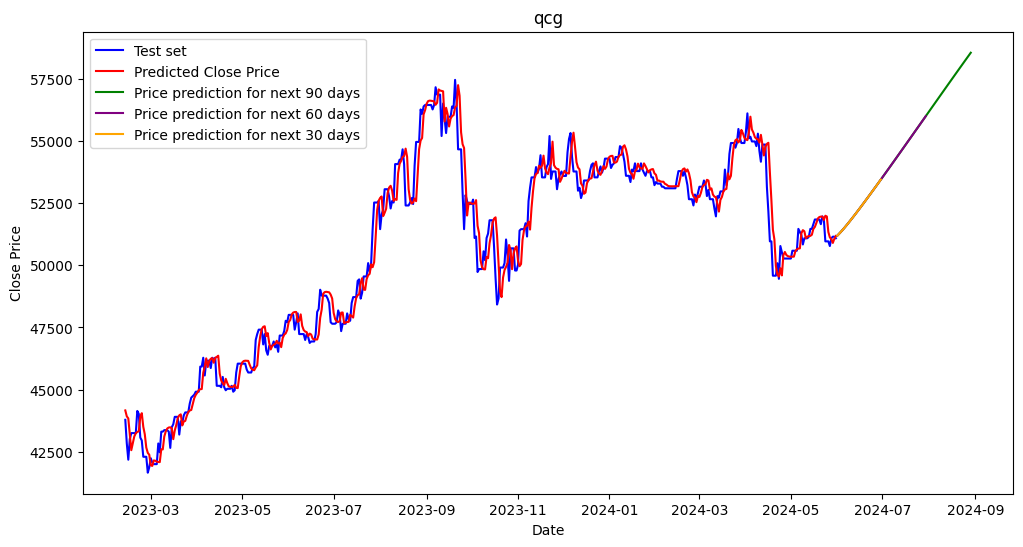
\includegraphics[width=1\textwidth]{bibliography/Figure/QCGGRU_9-1.png}
  \caption{GRU model's result with 9:1 splitting proportion}
  \label{fig:1}
  \end{minipage}
  \hfill
  \begin{minipage}{0.23\textwidth}
  \centering
  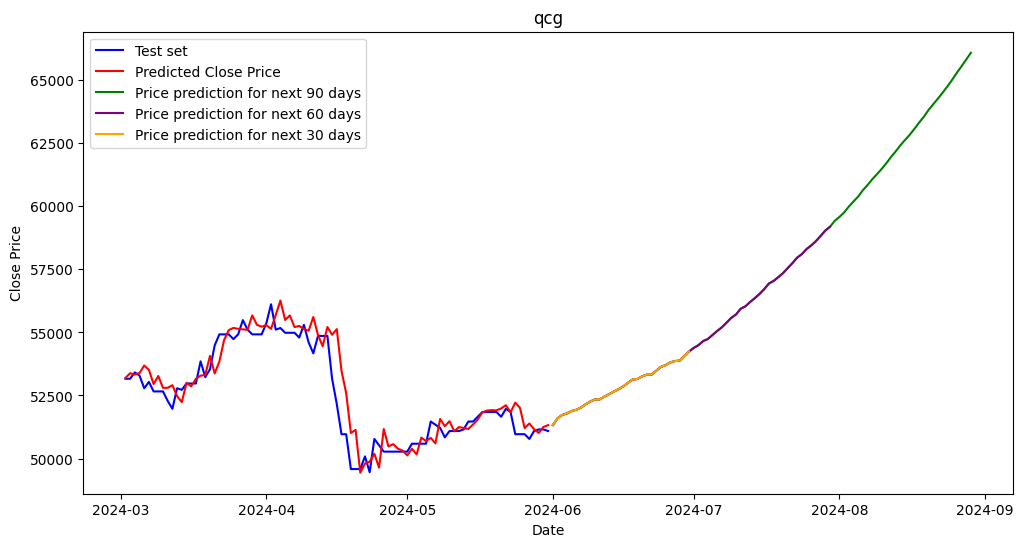
\includegraphics[width=1\textwidth]{bibliography/Figure/QCGRNN_9-1.png}
  \caption{RNN model's result with 9:1 splitting proportion}
  \label{fig:2}
  \end{minipage}
\end{figure}

\begin{figure}[H]
  \centering
  \begin{minipage}{0.23\textwidth}
  \centering
  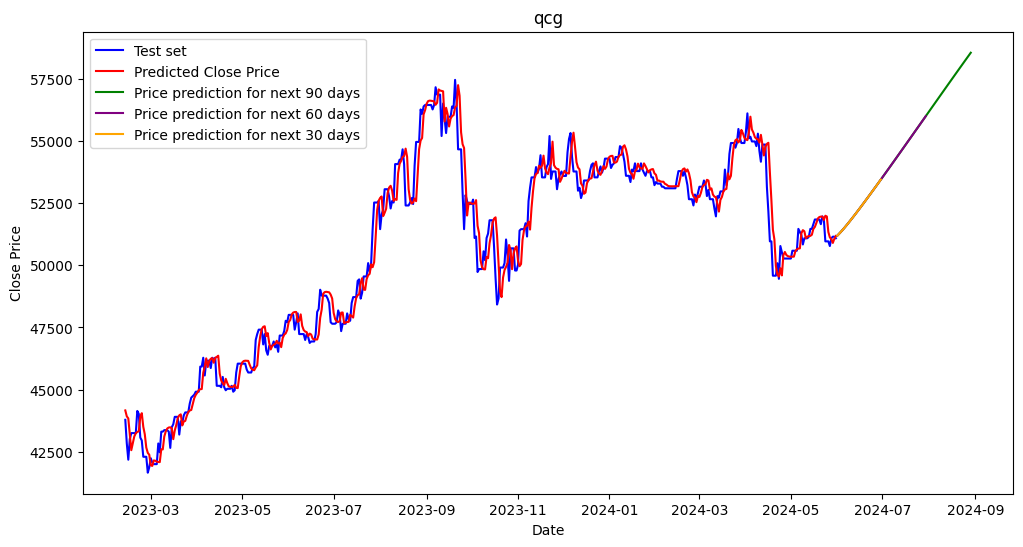
\includegraphics[width=1\textwidth]{bibliography/Figure/QCGGRU_9-1.png}
  \caption{GRU model's result with 9:1 splitting proportion}
  \label{fig:1}
  \end{minipage}
  \hfill
  \begin{minipage}{0.23\textwidth}
  \centering
  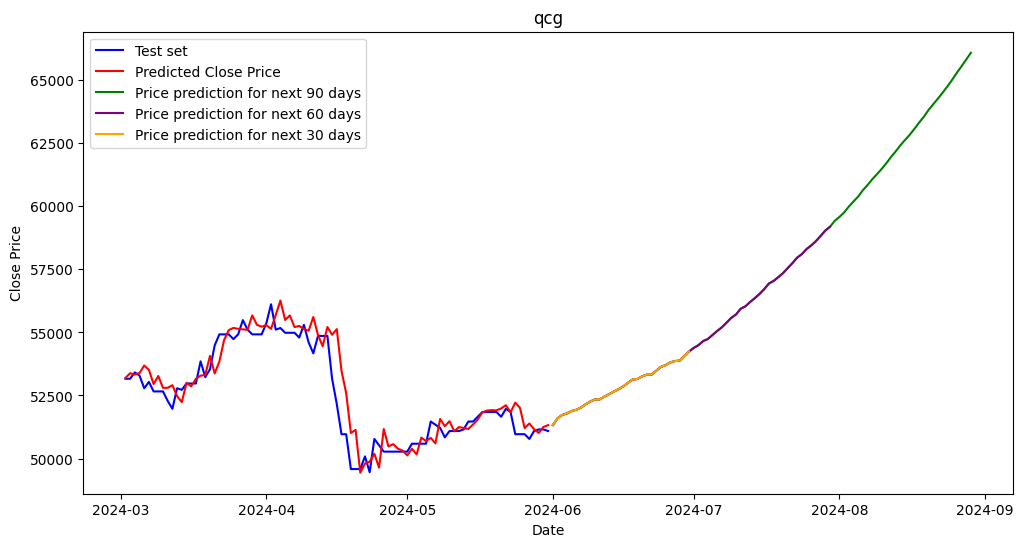
\includegraphics[width=1\textwidth]{bibliography/Figure/QCGRNN_9-1.png}
  \caption{RNN model's result with 9:1 splitting proportion}
  \label{fig:2}
  \end{minipage}
\end{figure}

\begin{figure}[H]
  \centering
  \begin{minipage}{0.23\textwidth}
  \centering
  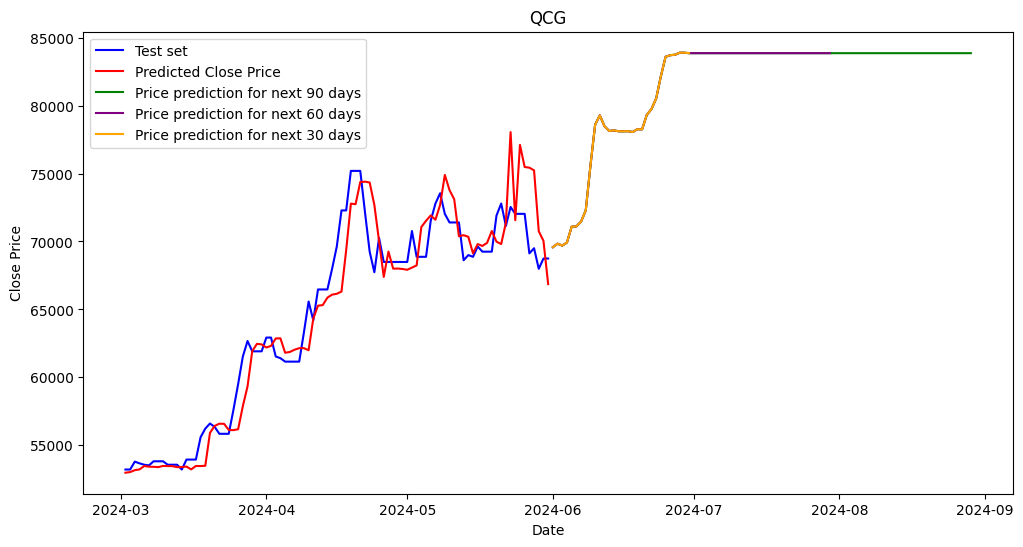
\includegraphics[width=1\textwidth]{bibliography/Figure/QCGRF_9-1.png}
  \caption{RF model's result with 9:1 splitting proportion}
  \label{fig:1}
  \end{minipage}
  \hfill
  \begin{minipage}{0.23\textwidth}
  \centering
  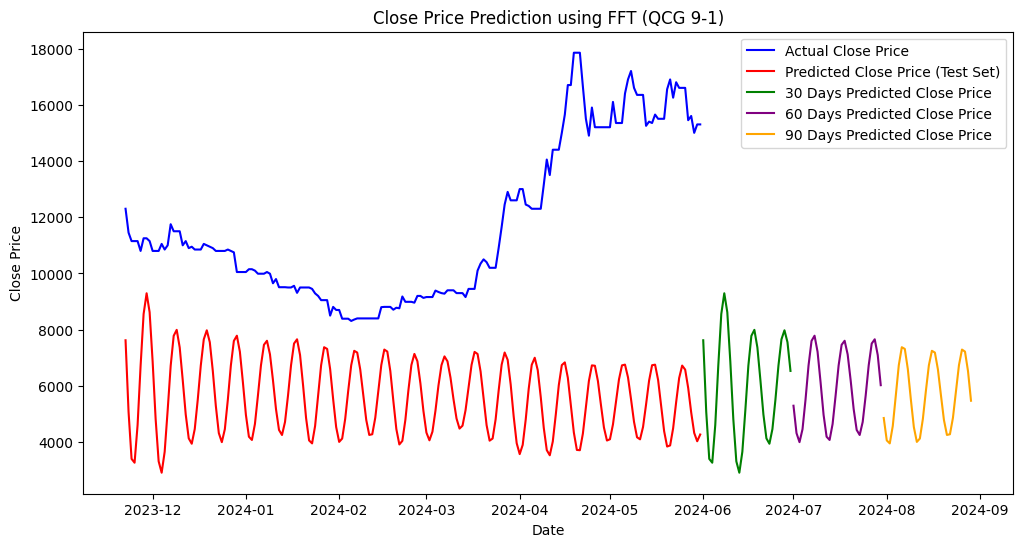
\includegraphics[width=1\textwidth]{bibliography/Figure/FFT_QCG(9-1).png}
  \caption{FFT model's result with 9:1 splitting proportion}
  \label{fig:2}
  \end{minipage}
\end{figure}

\section{Conclusion}
\subsection{Summary}
In the pursuit of forecasting stock prices, various methodologies have been explored, ranging from traditional statistical models to advanced machine learning algorithms. Among the examined models, Recurrent Neural Networks (RNN), Gated Recurrent Units (GRU), Long Short-Term Memory (LSTM), Random Forest, Fast Fourier Transform (FFT), TimesNet, and Auto Regressive Integrated Moving Average (ARIMA) stand out. Notably, RNN, GRU, LSTM, and Random Forest have emerged as the most promising and effective models for predicting stock prices.\\
The intricacies of stock price forecasting, rooted in the complexity and unpredictability of financial markets, demand models capable of capturing nuanced patterns and relationships within the data. Recurrent Neural Networks (RNN) excel at handling sequential data, offering robust predictions. Gated Recurrent Units (GRU) and Long Short-Term Memory (LSTM) models, with their enhanced ability to capture sequential dependencies, exhibit notable performance in stock price forecasting. Random Forest, with its ensemble learning approach, further refines predictive capabilities by combining multiple decision trees to provide collective insights\\
As evidenced by evaluation metrics such as RMSE, MAPE, and MAE, the RNN, GRU, LSTM, and Random Forest models consistently demonstrate superior performance across various aspects of forecasting accuracy. Their adaptability in managing the inherent uncertainties of stock markets positions them as formidable tools for investors and analysts seeking reliable predictions.\\
\subsection{Future Considerations}
The exploration of forecasting stock prices using Recurrent Neural Networks (RNN), Gated Recurrent Units (GRU), Long Short-Term Memory (LSTM), Random Forest, Fast Fourier Transform (FFT), TimesNet, and Auto Regressive Integrated Moving Average (ARIMA) models has yielded initial insights, yet the accuracy of these models remains a challenge. To enhance the predictive performance and applicability of these models, several future considerations are warranted:\\
\indent\textbullet\
Integrating more diverse and high-frequency data sources, such as social media sentiment, macroeconomic indicators, and real-time news feeds, could enrich the dataset, allowing models to capture a more comprehensive range of market dynamics and improve forecasting accuracy.
\indent\textbullet\
Utilizing and possibly developing more comprehensive evaluation metrics beyond RMSE, MAPE, and MAE to assess model performance can provide deeper insights into their effectiveness and areas needing improvement.
\\\indent\textbullet\
Developing hybrid models that combine the strengths of different approaches could yield better performance. For example, integrating the sequential learning capabilities of RNNs with the ensemble approach of Random Forests could result in models that better capture both short-term and long-term market patterns.

\section*{Acknowledgment}
\addcontentsline{toc}{section}{Acknowledgment}
Placeholder line

%% UNCOMMENT these lines below (and remove the 2 commands above) if you want to embed the bibliografy.
\begin{thebibliography}{00}
\bibitem{b1} Hind Daori, Alanoud Alanazi, Manar Alharthi, Ghaida Alzahrani
 ,  ''Predicting Stock Prices Using the Random ForestClassifier'', November, 14th, 2022.
\bibitem{b2} Hugo Souto, 2023, ''TimesNet for Realized Volatility Prediction
''.
\bibitem{b3} Bohumil Stádník, Jurgita Raudeliuniene, Vida Davidavičienė , 2016. Fourier Analysis For Stock Price Forecasting: Assumption And Evidence .

\end{thebibliography}
%%%%%%%%%%%%%%%


\EOD

\end{document}
